\documentclass[a4paper]{article}

\usepackage[margin=2.5cm]{geometry}
\usepackage[pdftex]{graphicx}
\usepackage[utf8]{inputenc}
\usepackage[T1]{fontenc}
\usepackage{textcomp}
\usepackage{babel}
\usepackage{amsmath, amssymb}
\usepackage[colorlinks=true,linkcolor=blue]{hyperref}
\usepackage{float}
\usepackage{mathrsfs}
%\usepackage{enumitem}
%% for identity function 1:
\usepackage{bbm}
%%For category theory diagrams:
%\usepackage{tikz-cd}
%%For code (e.g. python) in latex:
%\usepackage{listings}
%
%Usage: 
%\begin{lstlisting}[language=Python]
%\end{lstlisting}

\newcommand{\incfig}[2][1]{%
\def\svgwidth{#1\columnwidth}
\import{./figures/}{#2.pdf_tex}
}


% figure support
\usepackage{import}
\usepackage{xifthen}
\pdfminorversion=7
\usepackage{pdfpages}
\usepackage{transparent}

\pdfsuppresswarningpagegroup=1

\setlength\parindent{0pt}

\newcommand{\qed}{\tag*{$\blacksquare$}}
\newcommand{\qedwhite}{\hfill \ensuremath{\Box}}

%Inequalities
\newcommand{\cycsum}{\sum_{\mathrm{cyc}}}
\newcommand{\symsum}{\sum_{\mathrm{sym}}}
\newcommand{\cycprod}{\prod_{\mathrm{cyc}}}
\newcommand{\symprod}{\prod_{\mathrm{sym}}}

%Linear Algebra

\DeclareMathOperator{\Span}{span}
\DeclareMathOperator{\Ima}{Im}
\DeclareMathOperator{\diag}{diag}
\DeclareMathOperator{\Ker}{Ker}
\DeclareMathOperator{\ob}{ob}
\DeclareMathOperator{\Hom}{Hom}
\DeclareMathOperator{\sk}{sk}
\DeclareMathOperator{\Vect}{Vect}
\DeclareMathOperator{\Set}{Set}
\DeclareMathOperator{\Group}{Group}
\DeclareMathOperator{\Ring}{Ring}
\DeclareMathOperator{\Ab}{Ab}
\DeclareMathOperator{\Top}{Top}
\DeclareMathOperator{\Htpy}{Htpy}
\DeclareMathOperator{\Cat}{Cat}
\DeclareMathOperator{\CAT}{CAT}
\DeclareMathOperator{\Cone}{Cone}


%Row operations
\newcommand{\elem}[1]{% elementary operations
\xrightarrow{\substack{#1}}%
}

\newcommand{\lelem}[1]{% elementary operations (left alignment)
\xrightarrow{\begin{subarray}{l}#1\end{subarray}}%
}

%SS
\DeclareMathOperator{\supp}{supp}
\DeclareMathOperator{\Var}{Var}

%NT
\DeclareMathOperator{\ord}{ord}

%Alg
\DeclareMathOperator{\Rad}{Rad}
\DeclareMathOperator{\Jac}{Jac}

\DeclareMathAlphabet{\pazocal}{OMS}{zplm}{m}{n}
\newcommand{\unif}{\pazocal{U}}

\begin{document}
    \textbf{p. 178}\\
    \textbf{2:} Show that the elementary 1-cycles, mentioned in section 8.1,
    generates $Z_1 (K)$ for any complex $K$.\\
    \linebreak
    \textit{Solution:} Suppose $K$ is a simplicial complex. Let
    $\lambda = \sum \lambda_i (u_i, v_i) \in Z_1(K)$. We wish to show that
    there
    exist elementary $1$-cycles $\sigma_1, \ldots, \sigma_n$ such that
    $\lambda = \sum \sigma_i$.\\
    We can assume without loss of generality that
    the $\lambda_i$ are positive since otherwise we can replace
    $\lambda_i (u_i, v_i)$ by $(- \lambda_i) (v_i, u_i)$. Furthermore, suppose
    $(u_i, v_i) \neq (u_j, v_j)$ for all $i\neq j$.\\
    Denote $\delta_{i} := (u_i, v_i)$. Then starting from some $\delta_{i_0}$,
    since
    $0 = \partial \lambda = 
    \sum \lambda_j (v_j -u_j) $, we have that there must exist some
    $i_1$ with $u_{i_1} = v_{i_0}$. Then append
    $\delta_{i_0}. \delta_{i_1} $ which we will let denote the path
    $u_{i_0}, v_{i_0}, v_{i_1}$. Now, inductively, we can continue to do so
    until we eventually get some
    $\delta_{i_k}$ such that $\delta_{i_k} = \delta_{i_s}$ for some
    $0 \le s < k$. Then
    $\delta_{i_s}. \delta_{i_{s+1}}. \ldots . \delta_{i_{k-1}}$ is a closed
    chain, and we have effectively removed the vertices in this chain from
    $\partial \lambda$ since
    $\partial  \sum \delta_{i_h} 
    = \sum (v_{i_h}-u_{i_h})
    = v_{i_{k-1}} - u_{i_s}$, and since
    $(v_{i_{k-1}}, v_{i_k}) =(u_{i_k},v_{i_k}) = \delta_{i_k} 
    = \delta_{i_s} = (u_{i_s}, v_{i_s})$, we have
    $v_{i_{k-1}} = u_{i_s}$, so
    $\partial  \sum \delta_{i_h} = 0$, and further we thus have that
    the curve $u_{i_s}, v_{i_{s}}, v_{i_{s+1}}, \ldots, 
    v_{i_{k-1}}$ is a closed oriented polygonal curve in $K$. Furthermore,
    if it were not simple, then for some
     $i_s \le j < l \le i_{k-1}$, we would have
     $\delta_j = \delta_l$, however, by construction,
     $\delta_{i_{k-1}}$ was the first repeated $\delta$ in the chain
     $\delta_{i_0}, \ldots, \delta_{i_{k-1}}$, so this is not possible. Hence
     the curve is also simple. Taking a remaining
     $\delta \not\in  \delta_{i_s}. \ldots . \delta_{i_{k-1}}$ and repeat the
     procedure, we receive another chain. Now, since there is only a finite
     number of $\delta$ in $\lambda$, this procedure must end at some point.\\
     Denoting the chains in the end by  $\sigma_1, \ldots, \sigma_{N}$, we get
     $\lambda = \sum \sigma_{i=1}^{N}$ by construction, so
     $\lambda$ is a sum of elementary $1$-cycles.\\
     Hence $Z_1(K)$ is generated by elementary cycles.\\
     \linebreak

    \textbf{5:} As for problem 4, but this time orient all the triangles
    compatibly, with the exception of one of them which is given the
    'wrong' orientation.\\
    \textit{Solution:} We can orient the triangles as follows:
    \begin{figure}[H]
        \centering
        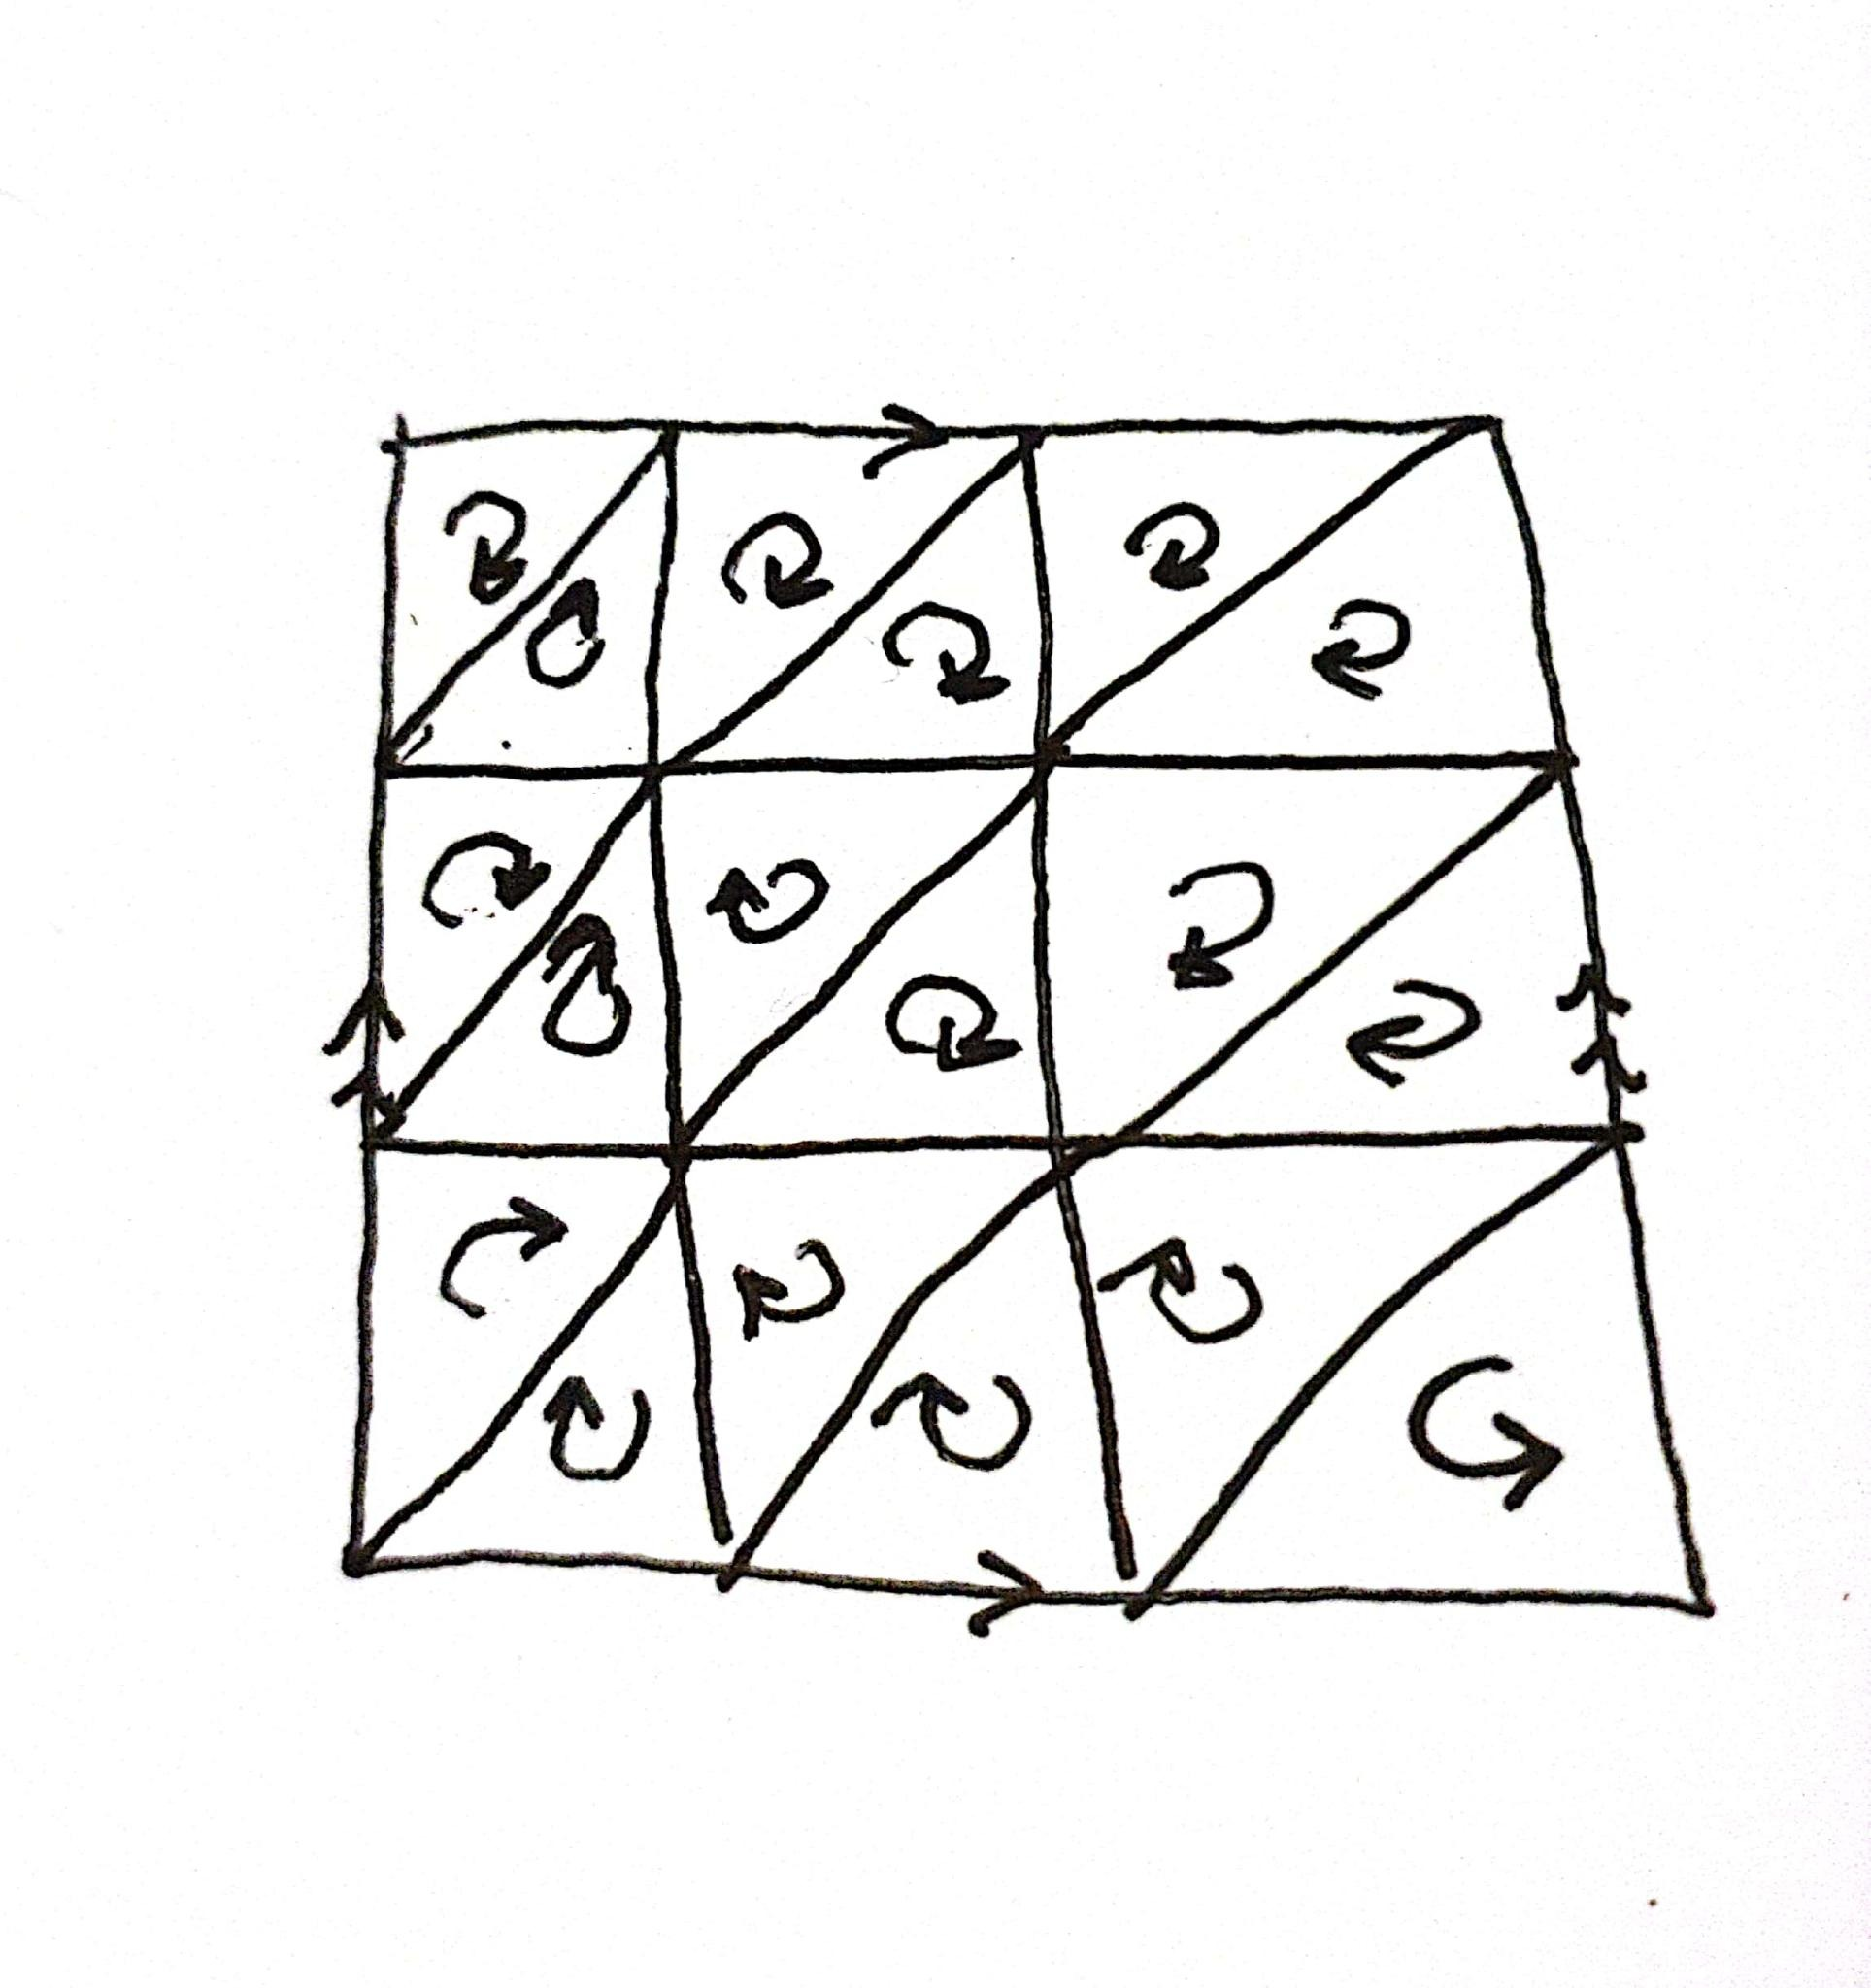
\includegraphics[width=0.5\textwidth]{5.jpeg}
        \label{fig:5-jpeg}
    \end{figure}
    Here, all triangles are oriented compatibly except for the bottom-right
    one, which has the 'wrong' orientation.\\
    Suppose we gave it the opposite orientation. Then
    the boundary of each edge of a triangle would cancel with the edge of
    another, so the boundary would be $0$. Now, switching the orientation of
    the bottom-right triangle back, give it an orientation
    $\left\{ v_0, v_1, v_2 \right\} $ with $v_0 < v_1 < v_2$, which is the
    wrong orientation. Then we have that
    in the 'right' orientation, the edges
    $\left[ v_2, v_1 \right] , \left[ v_1, v_0 \right] $ and
    $\left[ v_0, v_2 \right] $ with orientation, got cancelled, so there are
    neighboring edges
    $\left[ v_1, v_2 \right] , \left[ v_0 , v_1 \right] $ and
    $\left[ v_2, v_0 \right] $. Thus these do not get cancelled in the 'wrong'
    orientation either, so since all other edges still get cancelled, letting
    $A$ denote the collection of oriented triangles in the compatible
    orientations, we end up
    with the sum of the oriented triangles being
    $  \sum A + (v_2, v_1, v_0) - (v_0, v_1, v_2)
    = \sum A + 2 (v_2, v_1, v_0)$, so the boundary becomes
    $\partial \sum A + \partial \left( 2 (v_2, v_1, v_0) \right) 
    = 2 ( v_2, v_1 ) + 2 ( v_1, v_0 ) +
    2 ( v_0, v_2 ) 
    = 2 \partial \left[ v_0, v_2, v_1 \right] $, i.e. twice the boundary of the
    wrong triangle.























\end{document}
